
En este apartado, se aborda un análisis detallado de las plataformas y sistemas que actualmente exhiben un comportamiento similar al del sistema que se pretende desarrollar para 'BidMon Universe'. 

La realización de este análisis es muy importante, ya que proporciona una base sólida para la toma de decisiones estratégicas. Al examinar detenidamente tanto las ventajas como las desventajas de los sistemas existentes, se identifican estrategias exitosas y se reconocen posibles fallos 
o áreas susceptibles de mejora. Este enfoque no solo informa las decisiones de diseño y tecnología, sino que también las fundamenta en un conocimiento práctico y bien contextualizado. Así, se garantiza que el desarrollo de 'BidMon Universe' esté 
armonizado con las tendencias actuales y adopte las soluciones más efectivas y adecuadas para su propósito.

El objetivo del proyecto es permitir a los usuarios coleccionar cartas e intercambiarlas mediante subastas, específicamente cartas de Pokémon. Por esta razón, se ha llevado a cabo un análisis de sistemas similares enfocados en los siguientes puntos:
\begin{itemize}
    \item Sistemas de intercambio de cartas digitales: Se analizarán diversos sistemas de intercambio de cartas digitales, destacando su relevancia en el mercado y las funcionalidades que ofrecen.
    \item Sistemas de subastas en línea: Se evaluarán plataformas de subastas en línea, analizando sus ventajas y desventajas, con el objetivo de identificar las mejores prácticas aplicables a nuestro proyecto.
    \item El mercado de coleccionistas de Pokémon: Se estudiará la extensa base de seguidores y coleccionistas de cartas Pokémon, comprendiendo su comportamiento, preferencias y el impacto que tienen en el mercado de subastas.
\end{itemize}

\subsection{Análisis de sistemas de intercambio de cartas digitales}
En esta sección se analizarán los sistemas de intercambio de cartas digitales, como EA Sports FC, NBA 2K y LaLiga Fantasy, que permiten a los usuarios adquirir y vender cartas de jugadores. 
Aunque el sistema de coleccionismo de cartas puede variar según la plataforma del juego, todos comparten una serie de características comunes. Estas incluyen la posibilidad de pujar 
por un jugador o comprarlo directamente, la existencia de distintas rarezas de cartas y la inclusión de eventos especiales.

\subsubsection{EA Sports FC}
\coloredUnderline{\href{https://www.ea.com/es-es/games/ea-sports-fc}{EA Sports FC}} es una destacada franquicia de videojuegos de fútbol disponible en diversas plataformas. 
Este análisis se centrará en el modo de juego \coloredUnderline{\href{https://www.ea.com/es-es/games/fifa/fifa-23/ultimate-team/item-guide}{FIFA Ultimate Team}}, 
que busca transformar la interacción de los jugadores, permitiéndoles construir y gestionar su propio equipo de fútbol. Los usuarios pueden buscar jugadores en el mercado de transferibles, 
pujar por ellos o comprarlos directamente. Además, pueden incrementar el valor de sus jugadores completando desafíos y cambiar la apariencia de las cartas. 
Este modo incluye tarjetas de jugadores con distintas rarezas, haciendo que algunas sean más valiosas que otras.

Se estima que EA Sports FC ha generado más de 6.000 millones de dólares en ingresos netos entre 2020 y 2025\cite{sanmartin000MillonesDolares2021}. En 2020, 
los ingresos casi se triplicaron en comparación con 2015, demostrando un crecimiento exponencial. El informe anual de Electronic Arts para el año fiscal 2023\cite{ea2023} 
especifica que se generaron 7.426 millones de dólares en ingresos netos y revela que el modo Ultimate Team de FIFA 23 es el más popular de la franquicia, con más de 10 millones 
de jugadores activos mensuales, siendo una de las mayores fuentes de ingresos de la empresa. El informe también destaca la intención de continuar desarrollando este mercado 
mediante la incorporación de nuevas características para el modo Ultimate Team.

La popularidad de este modo de juego ha llevado a Electronic Arts a lanzar una aplicación móvil llamada \coloredUnderline{\href{https://apps.apple.com/es/app/ea-sports-fc-24-companion/id1127108818}{EA SPORTS FC™ 24 Companion}}, 
que permite a los usuarios gestionar su club de FIFA Ultimate Team desde dispositivos móviles. Los usuarios necesitan tener el juego FIFA 24 para utilizar la aplicación, 
la cual se conecta a la cuenta del usuario en el juego. Desde la aplicación, los usuarios pueden comprar sobres de cartas, gestionar su plantilla, 
comprar jugadores en el mercado de transferibles y pujar por jugadores en subastas para utilizarlos posteriormente en el juego.

En las siguientes figuras, se muestra la interfaz de usuario de EA SPORTS FC™ 24 Companion.

\begin{figure}[H]
    \centering
    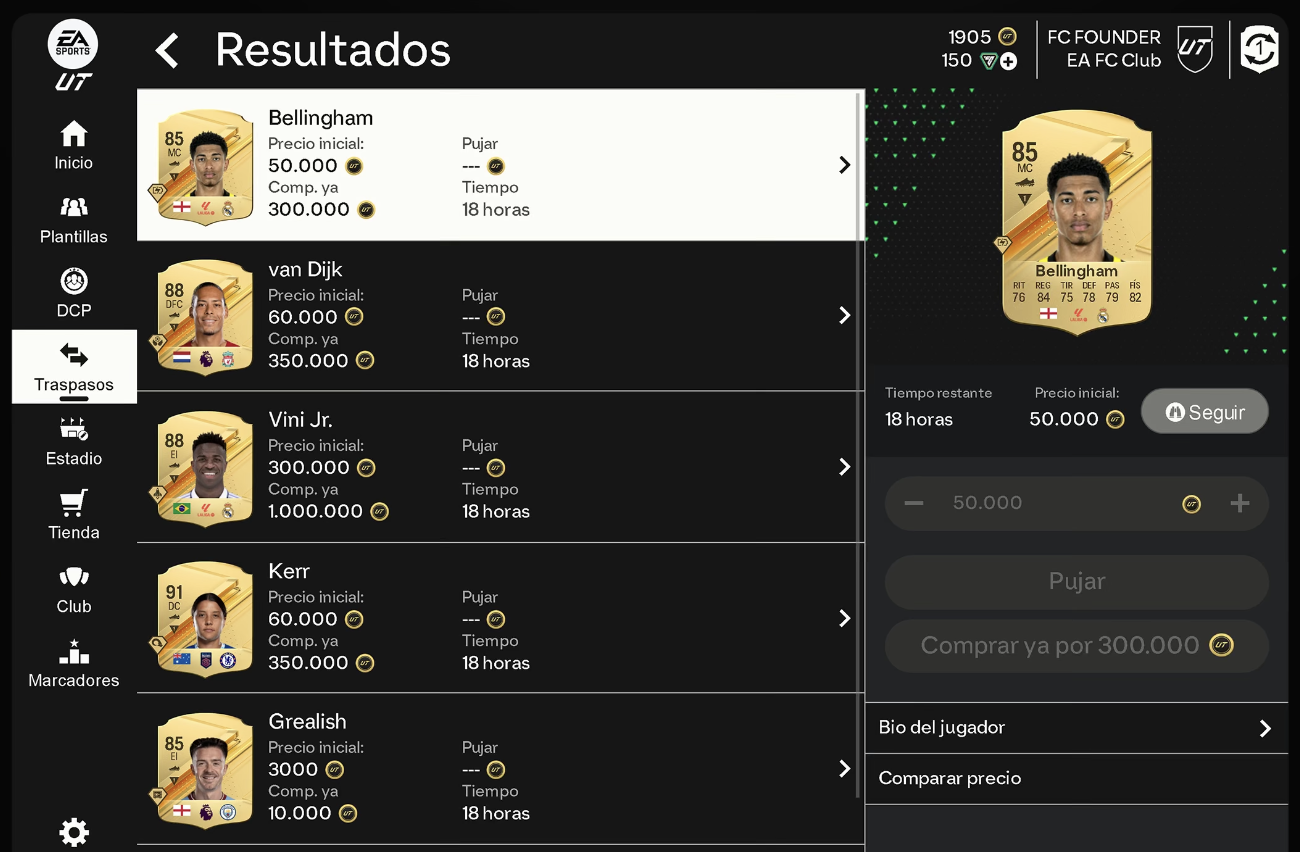
\includegraphics[width=0.7\textwidth]{figures/4-Estudio-viabilidad/4_FC_Companion.png}
    \caption{Página de traspasos de jugadores de EA SPORTS FC™ 24 Companion}
    \label{fig:ea_sports_fc_1}
    \hypertarget{fig:ea_sports_fc_1}{}
\end{figure}

\begin{figure}[H]
    \centering
    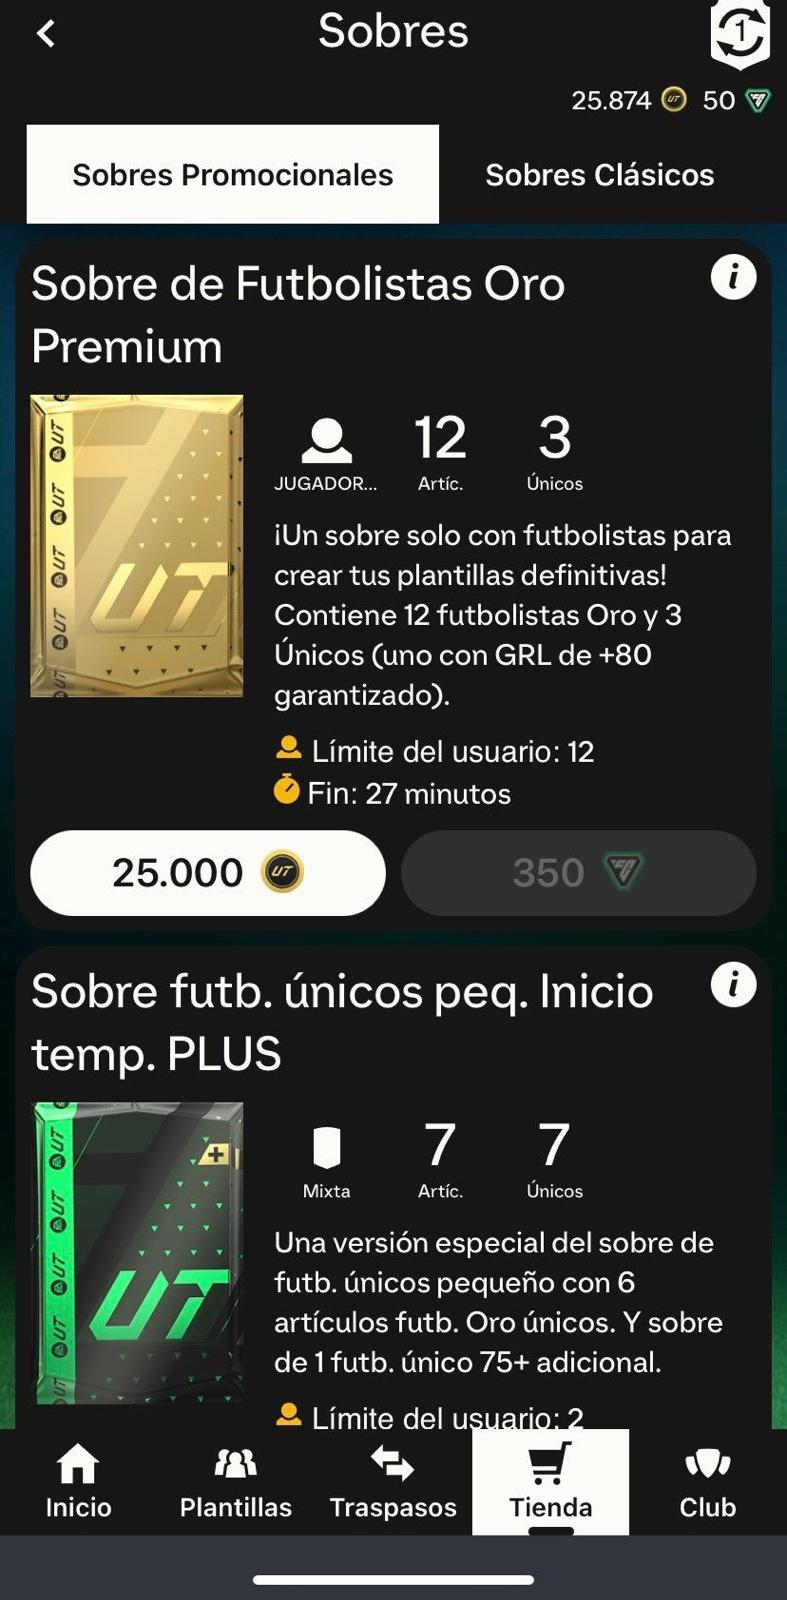
\includegraphics[width=0.3\textwidth]{figures/4-Estudio-viabilidad/4_FC_Companion2.jpeg}
    \caption{Página de compra de sobres de EA SPORTS FC™ 24 Companion}
    \label{fig:ea_sports_fc_2}
    \hypertarget{fig:ea_sports_fc_2}{}
\end{figure}

\subsubsubsection{Ventajas de EA Sports FC}
En el contexto de EA Sports FC, destacan las siguientes ventajas:
\begin{itemize}
    \item Los usuarios pueden marcar una carta para efectuar un seguimiento y recibir notificaciones en caso de una disminución en su precio.
    \item Se proporcionan estadísticas detalladas de cada carta, incluyendo su evolución de precio en las últimas semanas, así como los valores más bajos y más altos a los que se está vendiendo actualmente.
    \item Existe la opción de vender una carta directamente, evitando la necesidad de utilizar el sistema de subastas. 
    \item Cuenta con un buscador de ofertas que incorpora varios filtros.
    \item Los usuarios tienen la posibilidad de editar o cancelar sus pujas en curso.
    \item El sistema de subastas implementado opera bajo un mecanismo de puja ciega.
\end{itemize}

\subsubsubsection{Desventajas de EA Sports FC}
Sin embargo, es importante mencionar algunas desventajas de EA Sports FC, que incluyen:
\begin{itemize}
    \item Un número limitado de órdenes de canje simultáneas como, por ejemplo, el máximo de 25 permitido en EA Sports FC Mobile.
    \item Las pujas solo se pueden realizar por un valor igual o superior al establecido por el juego. 
\end{itemize}

\subsubsubsection{Ventajas del nuevo sistema respecto EA Sports FC}
El sistema en desarrollo presenta varias características que mejoran la experiencia del usuario en comparación con EA Sports FC.

\begin{itemize}
    \item El acceso a la aplicación es completamente gratuito.
    \item Ofrece una mayor personalización en el proceso de puja, brindando a los usuarios una experiencia más flexible y adaptada a sus preferencias.
    \item El usuario tiene la posibilidad de acceder a un histórico exhaustivo en el que se detallan todas las transacciones realizadas.
\end{itemize}

\subsubsection{LaLiga Fantasy}
\coloredUnderline{\href{https://laligafantasy.relevo.com/}{LaLiga Fantasy}} un juego basado en la liga de fútbol española, conocida como LaLiga. En este juego, los usuarios tienen la capacidad de crear equipos que se componen de jugadores cuyo rendimiento se correlaciona con el desempeño real en los partidos de LaLiga. Además, existe la posibilidad de competir por premios reales en determinadas instancias del juego.
El juego dispone de un mercado en el que los usuarios pueden vender o adquirir jugadores a través de un sistema de subastas, por lo que estamos ante un escenario similar al anterior.

A continuación, se muestra la interfaz de usuario de LaLiga Fantasy.
\begin{figure}[H]
    \centering
    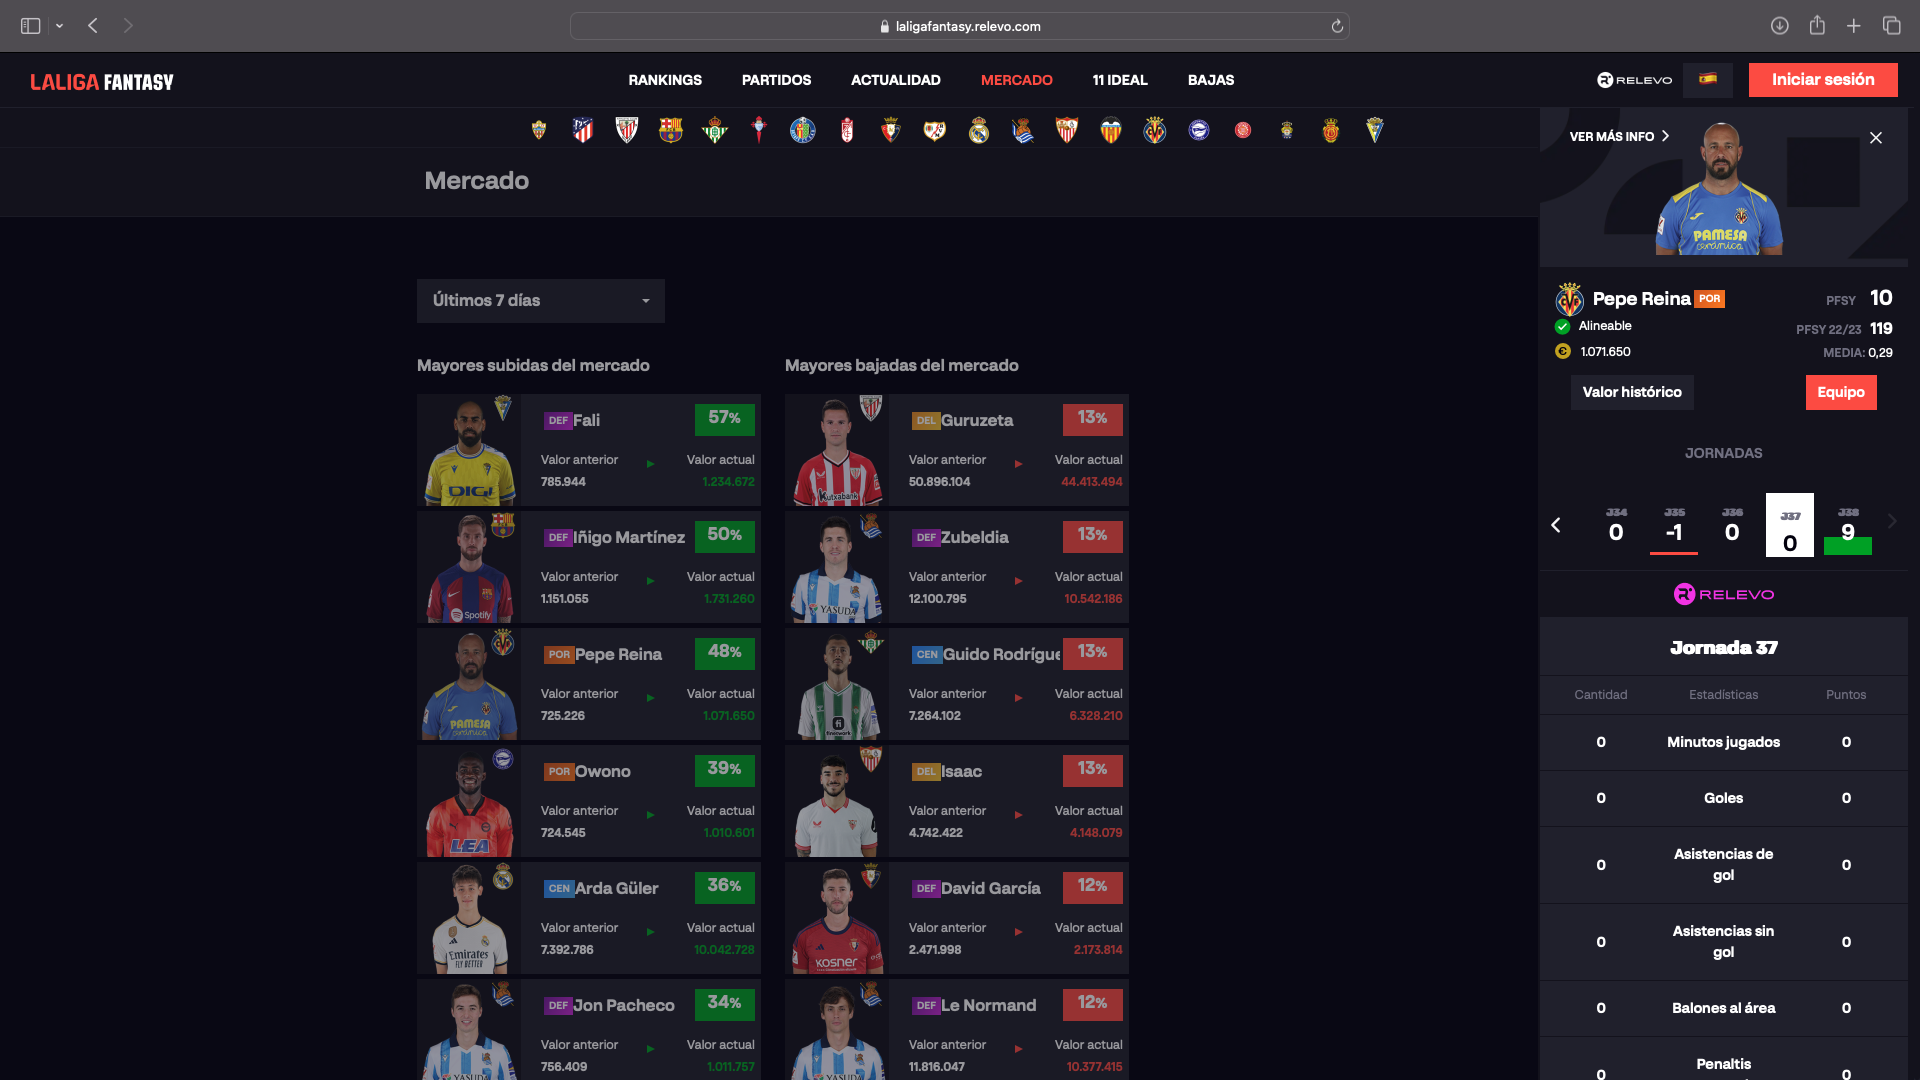
\includegraphics[width=0.7\textwidth]{figures/4-Estudio-viabilidad/4_LaLigaFantasy.png}
    \caption{Página de mercado de jugadores de LaLiga Fantasy}
    \label{fig:la_liga_fantasy}
    \hypertarget{fig:la_liga_fantasy}{}
\end{figure}

\subsubsubsection{Ventajas de LaLiga Fantasy}
Dentro del marco de LaLiga Fantasy, se destacan las siguientes características:
\begin{itemize}
    \item El juego renueva constantemente el mercado de transferibles.
    \item El juego cuenta con la capacidad de generar ofertas automáticas por los futbolistas que se encuentran en venta. Estas ofertas se establecen a partir de un valor aleatorio que oscila entre el valor de mercado del jugador, con un margen del 10\% tanto por encima como por debajo de dicho valor.
    \item Recientemente se ha incorporado el mercado de ``clausulazos'', donde los usuarios pueden adquirir un jugador pagando su cláusula, que será más elevada que el valor de mercado, sin tener que depender del propietario del jugador.
    \item Se pueden realizar ofertas por jugadores a otros usuarios.
\end{itemize}

\subsubsubsection{Desventajas de LaLiga Fantasy}
Se pueden identificar las siguientes desventajas:
\begin{itemize}
    \item La limitación a un máximo de 24 jugadores en la plantilla, lo que puede ocasionar la pérdida de oportunidades en subastas.
    \item La plataforma brinda escasa flexibilidad en lo que respecta a la personalización al momento de poner un jugador en venta.
\end{itemize}

\subsubsubsection{Ventajas del nuevo sistema respecto LaLiga Fantasy}
\begin{itemize}
    \item LaLiga Fantasy ofrece una suscripción de 0,99€/mes para poder jugar sin anuncios mientras que el sistema que se desarrollará carece de anuncios.
    \item Se proporciona un historial de transacciones completo para que los usuarios puedan rastrear las compras y ventas.
    \item Se implementa un sistema de subastas en tiempo real que, además, brinda una mayor personalización al usuario en aspectos como la duración de la subasta y los valores de venta, entre otros.
    \item Además de acceder al mercado, los usuarios tienen la opción de adquirir sobres de cartas, lo que añade un elemento de emoción a la aplicación.
\end{itemize}

\subsubsection{eBay}
\coloredUnderline{\href{https://www.ebay.es/}{eBay}} es una plataforma de comercio online que permite a los usuarios comprar y vender productos a través de subastas o ventas directas. Se puede encontrar una sección específica dedicada al coleccionismo, donde los usuarios pueden pujar por artículos de interés, como cartas.

En la siguiente figura, se muestra la interfaz de usuario de la sección de coleccionismo de cartas de eBay.
\begin{figure}[H]
    \centering
    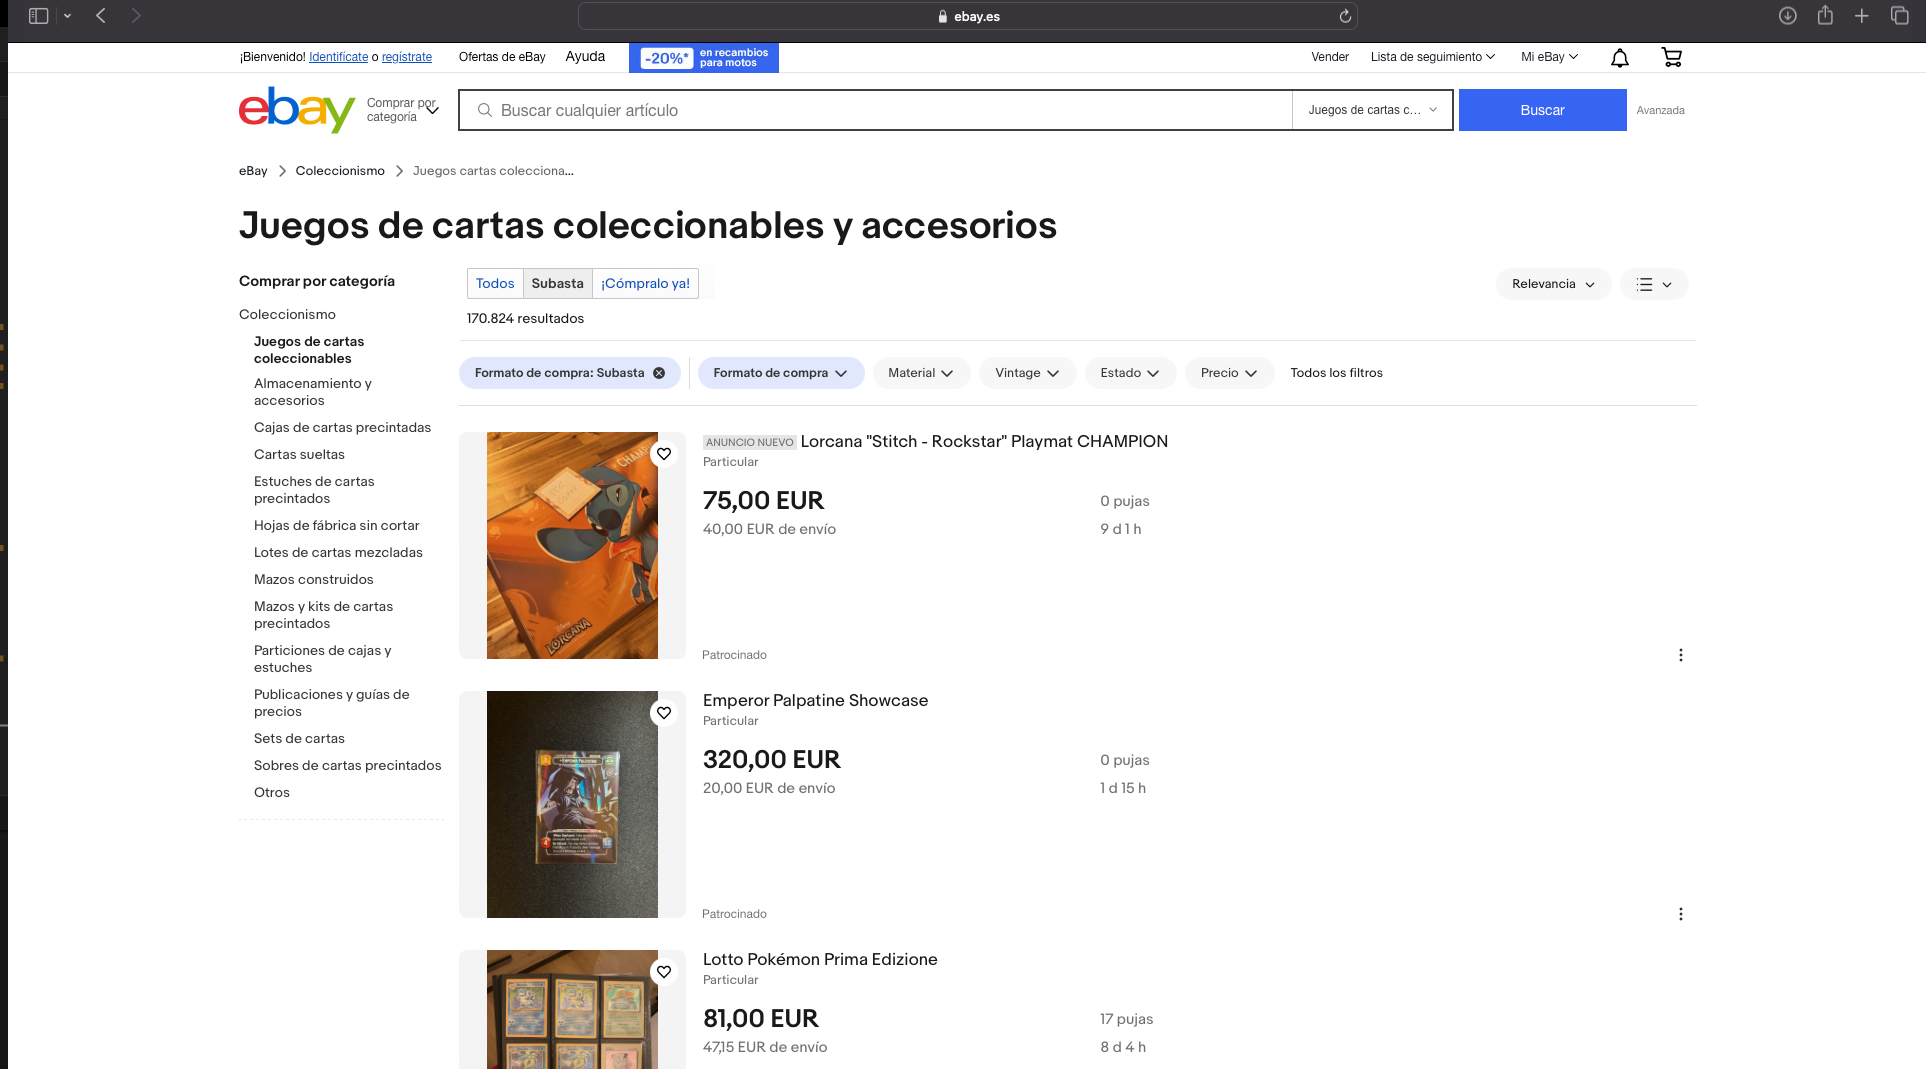
\includegraphics[width=0.9\textwidth]{figures/4-Estudio-viabilidad/4_Ebay.png}
    \caption{Página de subastas de la sección de coleccionismo de cartas de eBay}
    \label{fig:ebay}
    \hypertarget{fig:ebay}{}
\end{figure} 

\subsubsubsection{Ventajas de eBay}
Dentro del marco de LaLiga Fantasy, se destacan las siguientes características:
\begin{itemize}
    \item Para cada producto subastado, la plataforma ofrece la posibilidad de visualizar información detallada que incluye el número de pujas, la cantidad de pujadores, las retractaciones, el tiempo restante en la subasta, y proporciona un historial completo de las pujas realizadas en ese producto. Este historial incluye datos relevantes sobre las pujas, como su valor y la fecha en la que se efectuaron. Además, se brinda acceso a información pertinente sobre los pujadores involucrados.
    \item eBay proporciona a los usuarios la capacidad de configurar pujas automáticas. En este proceso, el comprador define el precio máximo que está dispuesto a pagar por el producto, y la plataforma aumenta automáticamente la oferta en su nombre, siempre que sea necesario, para mantener al comprador como el principal postor hasta alcanzar el límite previamente establecido.
    \item Los usuarios tienen la posibilidad de examinar el perfil del vendedor, explorar otros productos que este tenga en venta y establecer contacto directo con él.
    \item Como vendedor, la plataforma te brinda la capacidad de definir el valor inicial de la puja, decidir si deseas recibir ofertas, establecer la fecha de inicio de la subasta, determinar su duración y habilitar la opción de compra directa a un precio específico de tu elección.
\end{itemize}

\subsubsubsection{Desventajas de eBay}
A continuación, es posible señalar las siguientes desventajas:
\begin{itemize}
    \item La interfaz de usuario muestra una gran cantidad de información, lo que puede resultar confuso para alguien que no está acostumbrado a ella.
    \item Cuando se va a realizar una puja, no aparece una ventana emergente de confirmación de puja o similar por lo que es fácil introducir una puja errónea y, posteriormente, puede resultar complicado retirarla.
    \item Las subastas tienen incrementos de puja predefinidos, lo que significa que no puedes especificar un valor concreto por el que desees pujar.
\end{itemize}

\subsubsubsection{Ventajas del nuevo sistema respecto eBay}
\begin{itemize}
    \item El sistema en desarrollo presentará una interfaz simple e intuitiva, que proporcionará todos los datos esenciales para efectuar una puja con confianza, sin abrumar al usuario con una sobrecarga de información.
    \item El sistema que se desarrollará proporcionará al usuario información sobre las condiciones para retirar una puja antes de su confirmación.
\end{itemize}